\documentclass[aspectratio=169,12pt]{beamer}
\usetheme{Madrid}
\usecolortheme{dolphin}
\usefonttheme{professionalfonts}
\setbeamertemplate{navigation symbols}{}
\setbeamertemplate{footline}{}

\usepackage[T1]{fontenc}
\usepackage[utf8]{inputenc}
\usepackage{graphicx}
\usepackage{amsmath,amssymb}
\usepackage{hyperref}
\usepackage{siunitx}
\usepackage{physics}
\usepackage{tikz}
\usetikzlibrary{angles,quotes}

\title[Nombres Complexes]{Introduction aux Nombres Complexes}
\author{JAMOTTE Maxime, SCHOONEN Cédric}
\institute{Digital Learning Hub}
\date{}

\begin{document}

\begin{frame}
  \titlepage
\end{frame}

\begin{frame}{Table des matières}
  \tableofcontents
\end{frame}

\section{Motivation}

\begin{frame}{Problème: racine de nombres négatifs}
  Dans l'ensemble des nombres réels $\mathbb{R}$, la racine carrée de nombres négatifs n'existe pas:
  \[
    \sqrt{-1} \quad \text{n'a pas de solution dans } \mathbb{R}
  \]
  
  \bigskip
  \textbf{Solution:} On introduit un nouveau nombre $i$ tel que:
  \[
    i^2 = -1 \qquad \text{ou} \qquad i = \sqrt{-1}
  \]
\end{frame}

\begin{frame}{Construction des nombres complexes}
  À partir de $i$, on peut construire de nouveaux nombres:
  
  \bigskip
  On peut multiplier $i$ par un réel:
  \[
    y \cdot i \qquad \text{avec } y \in \mathbb{R}
  \]
  
  \bigskip
  On peut additionner avec un autre réel:
  \[
    z = x + yi \qquad \text{avec } x, y \in \mathbb{R}
  \]
  
  \bigskip
  Ceci est la \textbf{forme générale d'un nombre complexe}.
\end{frame}

\begin{frame}{Trois représentations}
  Un nombre complexe $z$ peut s'écrire de plusieurs manières:
  
  \bigskip
  \textbf{Forme cartésienne:}
  \[
    z = x + yi
  \]
  
  \textbf{Forme vectorielle:}
  \[
    z = (x, y)
  \]
  
  \textbf{Forme polaire:}
  \[
    z = \rho e^{i\theta}
  \]
\end{frame}

\section{Représentation cartésienne}

\begin{frame}{Représentation cartésienne}
  Un nombre complexe s'écrit:
  \[
    z = x + yi
  \]
  où $x$ est la partie réelle et $y$ la partie imaginaire.
  
  \bigskip
  \begin{center}
  \begin{tikzpicture}[scale=1.2]
    \draw[->] (-0.5,0) -- (3.5,0) node[right] {Re};
    \draw[->] (0,-0.5) -- (0,2.5) node[above] {Im};
    \draw[->,thick,blue] (0,0) -- (2.5,1.5) node[midway,above left] {$z$};
    \draw[dashed] (2.5,0) node[below] {$x$} -- (2.5,1.5);
    \draw[dashed] (0,1.5) node[left] {$y$} -- (2.5,1.5);
    \filldraw[blue] (2.5,1.5) circle (2pt) node[above right] {$x + yi$};
  \end{tikzpicture}
  \end{center}
\end{frame}

\begin{frame}{Addition et soustraction}
  L'addition se fait composante par composante:
  \[
    (x_1 + y_1 i) + (x_2 + y_2 i) = (x_1+x_2) + (y_1+y_2)i
  \]
  
  \begin{center}
  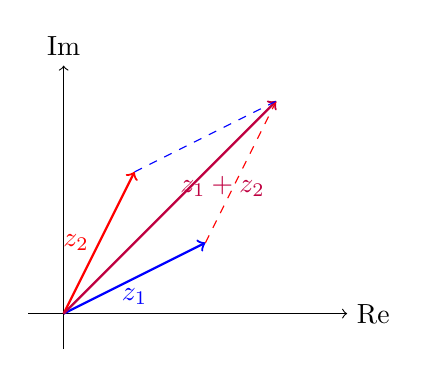
\begin{tikzpicture}[scale=0.9]
    \draw[->] (-0.5,0) -- (4,0) node[right] {Re};
    \draw[->] (0,-0.5) -- (0,3.5) node[above] {Im};
    \draw[->,thick,blue] (0,0) -- (2,1) node[midway,below] {$z_1$};
    \draw[->,thick,red] (0,0) -- (1,2) node[midway,left] {$z_2$};
    \draw[->,thick,purple] (0,0) -- (3,3) node[midway,above right] {$z_1+z_2$};
    \draw[dashed,red] (2,1) -- (3,3);
    \draw[dashed,blue] (1,2) -- (3,3);
  \end{tikzpicture}
  \end{center}
  
  Géométriquement: addition vectorielle.
\end{frame}

\begin{frame}{Multiplication en forme cartésienne}
  La multiplication utilise la propriété $i^2 = -1$:
  \begin{align*}
    (x_1 + y_1 i)(x_2 + y_2 i) &= x_1 x_2 + x_1 y_2 i + y_1 i x_2 + y_1 y_2 i^2 \\
    &= x_1 x_2 + x_1 y_2 i + y_1 x_2 i + y_1 y_2 (-1) \\
    &= (x_1 x_2 - y_1 y_2) + (x_1 y_2 + y_1 x_2)i
  \end{align*}
  
  \bigskip
  \textbf{Exemple:}
  \[
    (2 + 3i)(1 + 4i) = (2 \cdot 1 - 3 \cdot 4) + (2 \cdot 4 + 3 \cdot 1)i = -10 + 11i
  \]
\end{frame}

\section{Représentation vectorielle}

\begin{frame}{Représentation vectorielle}
  On peut voir un nombre complexe comme un vecteur dans le plan:
  \[
    z = x + yi \quad \longleftrightarrow \quad \vec{z} = \begin{pmatrix} x \\ y \end{pmatrix}
  \]
  
  \begin{center}
  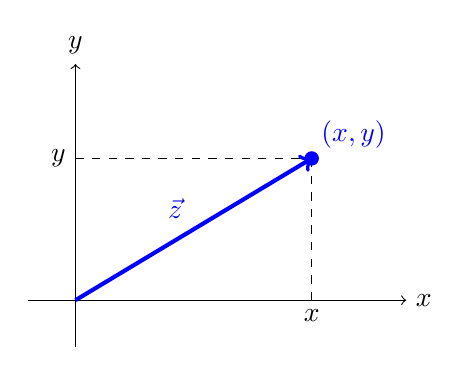
\begin{tikzpicture}[scale=1.2]
    \draw[->] (-0.5,0) -- (3.5,0) node[right] {$x$};
    \draw[->] (0,-0.5) -- (0,2.5) node[above] {$y$};
    \draw[->,thick,blue,line width=1.5pt] (0,0) -- (2.5,1.5) node[midway,above left] {$\vec{z}$};
    \draw[dashed] (2.5,0) node[below] {$x$} -- (2.5,1.5);
    \draw[dashed] (0,1.5) node[left] {$y$} -- (2.5,1.5);
    \filldraw[blue] (2.5,1.5) circle (2pt) node[above right] {$(x, y)$};
  \end{tikzpicture}
  \end{center}
\end{frame}

\begin{frame}{Addition et soustraction vectorielle}
  L'addition de deux complexes correspond à l'addition vectorielle:
  \[
    \begin{pmatrix} x_1 \\ y_1 \end{pmatrix} + \begin{pmatrix} x_2 \\ y_2 \end{pmatrix} = \begin{pmatrix} x_1 + x_2 \\ y_1 + y_2 \end{pmatrix}
  \]
  
  \begin{center}
  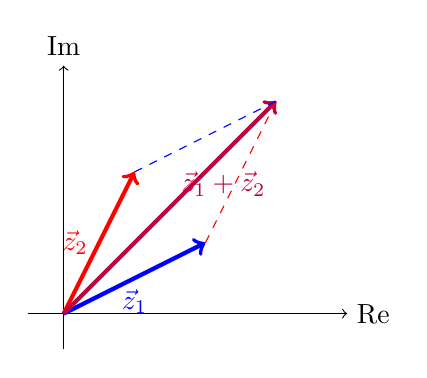
\begin{tikzpicture}[scale=0.9]
    \draw[->] (-0.5,0) -- (4,0) node[right] {Re};
    \draw[->] (0,-0.5) -- (0,3.5) node[above] {Im};
    \draw[->,thick,blue,line width=1.5pt] (0,0) -- (2,1) node[midway,below] {$\vec{z}_1$};
    \draw[->,thick,red,line width=1.5pt] (0,0) -- (1,2) node[midway,left] {$\vec{z}_2$};
    \draw[->,thick,purple,line width=1.5pt] (0,0) -- (3,3) node[midway,above right] {$\vec{z}_1+\vec{z}_2$};
    \draw[dashed,red] (2,1) -- (3,3);
    \draw[dashed,blue] (1,2) -- (3,3);
  \end{tikzpicture}
  \end{center}
\end{frame}

\begin{frame}{Multiplication vectorielle}
  La multiplication de complexes transforme les vecteurs:
  \[
    z_1 \cdot z_2 = (x_1 x_2 - y_1 y_2) + (x_1 y_2 + y_1 x_2)i
  \]
  
  correspond à la transformation:
  \[
    \begin{pmatrix} x_1 & -y_1 \\ y_1 & x_1 \end{pmatrix} \begin{pmatrix} x_2 \\ y_2 \end{pmatrix} = \begin{pmatrix} x_1 x_2 - y_1 y_2 \\ x_1 y_2 + y_1 x_2 \end{pmatrix}
  \]
  
  \bigskip
  Cette matrice effectue une \textbf{rotation} et un \textbf{étirement}.
\end{frame}

\section{Lien avec les rotations}

\begin{frame}{Multiplication par $i$}
  Que se passe-t-il quand on multiplie un nombre complexe par $i$?
  \[
    i \cdot (x + yi) = ix + yi^2 = ix - y = -y + xi
  \]
  
  \begin{center}
  \begin{tikzpicture}[scale=1.2]
    \draw[->] (-2.5,0) -- (2.5,0) node[right] {Re};
    \draw[->] (0,-0.5) -- (0,2.5) node[above] {Im};
    \draw[->,thick,blue] (0,0) -- (2,1) node[midway,below right] {$z$};
    \draw[->,thick,red] (0,0) -- (-1,2) node[midway,above left] {$iz$};
    \draw[->] (0.7,0) arc (0:90:0.7);
    \node at (0.5,0.5) {$90°$};
  \end{tikzpicture}
  \end{center}
  
  Multiplier par $i$ = \textbf{rotation de 90° dans le sens anti-horaire}.
\end{frame}

\begin{frame}{Multiplication par $2+2i$}
  Considérons la multiplication par $2 + 2i$:
  \[
    (2 + 2i)(x + yi) = (2x - 2y) + (2x + 2y)i
  \]
  
  \begin{center}
  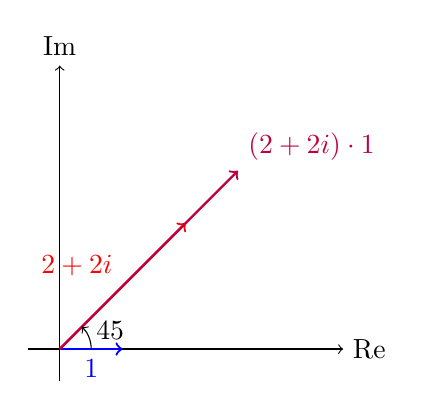
\begin{tikzpicture}[scale=0.8]
    \draw[->] (-0.5,0) -- (4.5,0) node[right] {Re};
    \draw[->] (0,-0.5) -- (0,4.5) node[above] {Im};
    \draw[->,thick,blue] (0,0) -- (1,0) node[midway,below] {$1$};
    \draw[->,thick,red] (0,0) -- (2,2) node[midway,above left] {$2+2i$};
    \draw[->,thick,purple] (0,0) -- (2.83,2.83) node[above right] {$(2+2i)\cdot 1$};
    \draw[->] (0.5,0) arc (0:45:0.5);
    \node at (0.8,0.3) {$45°$};
  \end{tikzpicture}
  \end{center}
  
  \textbf{Rotation de 45°} et \textbf{allongement} par un facteur $|2+2i| = 2\sqrt{2}$.
\end{frame}

\begin{frame}{Le module}
  Le \textbf{module} (ou norme) d'un nombre complexe mesure la longueur du vecteur $(x, y)$:
  \[
    |z| = \sqrt{x^2 + y^2}
  \]
  
  \begin{center}
  \begin{tikzpicture}[scale=1.2]
    \draw[->] (-0.5,0) -- (3.5,0) node[right] {Re};
    \draw[->] (0,-0.5) -- (0,2.5) node[above] {Im};
    \draw[->,thick,blue,line width=1.5pt] (0,0) -- (2.5,1.5) node[midway,above left] {$|z|$};
    \draw[dashed] (2.5,0) node[below] {$x$} -- (2.5,1.5);
    \draw[dashed] (0,1.5) node[left] {$y$} -- (2.5,1.5);
    \draw (0.5,0) arc (0:31:0.5);
    \node at (0.8,0.2) {$\theta$};
  \end{tikzpicture}
  \end{center}
\end{frame}

\begin{frame}{Interprétation trigonométrique}
  La trigonométrie nous permet d'interpréter $z = x + iy$ comme:
  \[
    z = |z| \left[ \cos(\theta) + i\sin(\theta) \right]
  \]
  
  où $\theta$ est l'angle que fait le vecteur avec l'axe réel.
  
  \bigskip
  Relations:
  \[
    x = |z| \cos(\theta) \qquad y = |z| \sin(\theta)
  \]
  \[
    |z| = \sqrt{x^2 + y^2} \qquad \theta = \arctan\left(\frac{y}{x}\right)
  \]
\end{frame}

\section{Complexe conjugué et division}

\begin{frame}{Division comme rotation inverse}
  Ayant compris les multiplications comme des rotations, il est plus facile de comprendre les divisions:
  
  \bigskip
  \textbf{Division = rotation inverse}
  
  \bigskip
  Pour inverser une rotation d'angle $\theta$, on effectue une rotation d'angle $-\theta$.
  
  \bigskip
  Ceci nous amène au concept de \textbf{complexe conjugué}.
\end{frame}

\begin{frame}{Le complexe conjugué}
  Le conjugué de $z = x + iy$ est noté $z^*$ (ou $\bar{z}$):
  \[
    z^* = x - iy
  \]
  
  En notation trigonométrique:
  \[
    z = |z|[\cos(\theta) + i\sin(\theta)] \quad \Rightarrow \quad z^* = |z|[\cos(\theta) - i\sin(\theta)]
  \]
  
  \bigskip
  Le conjugué correspond à une \textbf{réflexion par rapport à l'axe réel}:
  \[
    \theta \rightarrow -\theta
  \]
\end{frame}

\begin{frame}{Propriétés du conjugué}
  \begin{center}
  \begin{tikzpicture}[scale=1.2]
    \draw[->] (-0.5,0) -- (3.5,0) node[right] {Re};
    \draw[->] (0,-2,0) -- (0,2) node[above] {Im};
    \draw[->,thick,blue] (0,0) -- (2.5,1.5) node[midway,above left] {$z$};
    \draw[->,thick,red] (0,0) -- (2.5,-1.5) node[midway,below left] {$z^*$};
    \draw[dashed] (2.5,1.5) -- (2.5,-1.5);
    \draw (0.7,0) arc (0:31:0.7);
    \draw (0.7,0) arc (0:-31:0.7);
    \node at (1,0.3) {$\theta$};
    \node at (1,-0.3) {$-\theta$};
  \end{tikzpicture}
  \end{center}
  
  Propriété importante:
  \[
    z \cdot z^* = (x + iy)(x - iy) = x^2 + y^2 = |z|^2
  \]
\end{frame}

\begin{frame}{Division de nombres complexes}
  Pour diviser par un nombre complexe, on multiplie par le conjugué divisé par le module au carré:
  \[
    \frac{1}{z} = \frac{z^*}{|z|^2} = \frac{x - iy}{x^2 + y^2}
  \]
  
  \bigskip
  Pour diviser deux complexes:
  \[
    \frac{z_1}{z_2} = \frac{z_1 \cdot z_2^*}{|z_2|^2}
  \]
\end{frame}

\begin{frame}{Division détaillée en notation $x + iy$}
  Calculons $\frac{z_1}{z_2} = \frac{x_1 + iy_1}{x_2 + iy_2}$:
  
  \begin{align*}
    \frac{x_1 + iy_1}{x_2 + iy_2} &= \frac{(x_1 + iy_1)(x_2 - iy_2)}{(x_2 + iy_2)(x_2 - iy_2)} \\
    &= \frac{(x_1 x_2 + y_1 y_2) + i(y_1 x_2 - x_1 y_2)}{x_2^2 + y_2^2} \\
    &= \frac{x_1 x_2 + y_1 y_2}{x_2^2 + y_2^2} + i\frac{y_1 x_2 - x_1 y_2}{x_2^2 + y_2^2}
  \end{align*}
\end{frame}

\section{Représentation polaire}

\begin{frame}{Notation exponentielle}
  Un nombre complexe en notation polaire s'écrit:
  \[
    z = |z| e^{i\theta}
  \]
  
  Cette notation est \textbf{naturelle} car elle transforme les multiplications en sommes sur les angles (qu'on appelle aussi \textbf{phases}):
  \[
    z_1 \cdot z_2 = |z_1| e^{i\theta_1} \cdot |z_2| e^{i\theta_2} = |z_1||z_2| e^{i(\theta_1 + \theta_2)}
  \]
  
  \begin{itemize}
    \item Les modules se \textbf{multiplient}
    \item Les phases s'\textbf{additionnent}
  \end{itemize}
\end{frame}

\begin{frame}{Illustration: multiplication en forme polaire}
  \begin{center}
  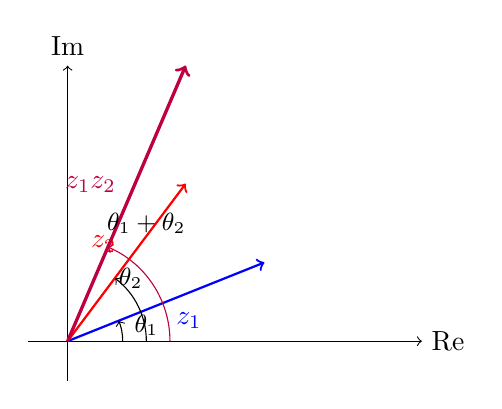
\begin{tikzpicture}[scale=1.0]
    \draw[->] (-0.5,0) -- (4.5,0) node[right] {Re};
    \draw[->] (0,-0.5) -- (0,3.5) node[above] {Im};
    \draw[->,thick,blue] (0,0) -- (2.5,1) node[midway,below right] {$z_1$};
    \draw[->,thick,red] (0,0) -- (1.5,2) node[midway,above left] {$z_2$};
    \draw[->,thick,purple,line width=1.2pt] (0,0) -- (1.5,3.5) node[midway,above left] {$z_1 z_2$};
    \draw[->] (0.7,0) arc (0:22:0.7);
    \node at (1,0.2) {\small $\theta_1$};
    \draw[->] (1.0,0) arc (0:53:1.0);
    \node at (0.8,0.8) {\small $\theta_2$};
    \draw[->,purple] (1.3,0) arc (0:67:1.3);
    \node at (1.0,1.5) {\small $\theta_1+\theta_2$};
  \end{tikzpicture}
  \end{center}
\end{frame}

\begin{frame}{Formule d'Euler}
  La \textbf{formule d'Euler} établit le lien entre l'exponentielle et les fonctions trigonométriques:
  \[
    e^{i\theta} = \cos(\theta) + i\sin(\theta)
  \]
  
  \bigskip
  Cas particuliers remarquables:
  \begin{align*}
    e^{i\pi} &= -1 \qquad \text{(identité d'Euler: } e^{i\pi} + 1 = 0 \text{)} \\
    e^{i\pi/2} &= i \\
    e^{2i\pi} &= 1
  \end{align*}
\end{frame}

\begin{frame}{Séparation module/phase}
  La notation $z = |z| e^{i\theta}$ sépare de manière élégante:
  
  \bigskip
  \begin{itemize}
    \setlength{\itemsep}{1em}
    \item Le \textbf{module} $|z|$: l'amplitude, la longueur
    \item La \textbf{phase} $\theta$: l'angle, la direction
  \end{itemize}
  
  \bigskip
  Cette séparation est particulièrement utile en physique quantique où:
  \begin{itemize}
    \item $|z|^2$ donne la probabilité
    \item $\theta$ donne la phase quantique
  \end{itemize}
\end{frame}

\begin{frame}{Opérations en notation polaire}
  \textbf{Multiplication:}
  \[
    z_1 \cdot z_2 = (|z_1| e^{i\theta_1})(|z_2| e^{i\theta_2}) = |z_1||z_2| \, e^{i(\theta_1+\theta_2)}
  \]
  
  \textbf{Division:}
  \[
    \frac{z_1}{z_2} = \frac{|z_1| e^{i\theta_1}}{|z_2| e^{i\theta_2}} = \frac{|z_1|}{|z_2|} \, e^{i(\theta_1-\theta_2)}
  \]
  
  \textbf{Puissance:}
  \[
    z^n = (|z| e^{i\theta})^n = |z|^n e^{in\theta}
  \]
  
  \textbf{Racine n-ième:}
  \[
    \sqrt[n]{z} = |z|^{1/n} e^{i\theta/n}
  \]
\end{frame}

\begin{frame}{Racines de l'unité}
  Les racines n-ièmes de l'unité sont les solutions de $z^n = 1$:
  \[
    \omega_k = e^{2\pi i k/n} \qquad k = 0, 1, 2, \ldots, n-1
  \]
  
  \bigskip
  Elles forment un polygone régulier à $n$ sommets dans le plan complexe.
  
  \begin{center}
  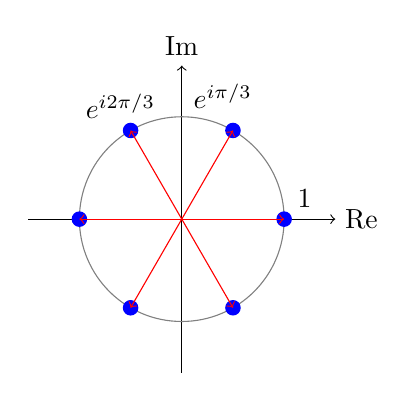
\begin{tikzpicture}[scale=1.3]
    \draw[->] (-1.5,0) -- (1.5,0) node[right] {Re};
    \draw[->] (0,-1.5) -- (0,1.5) node[above] {Im};
    \draw[gray] (0,0) circle (1);
    \foreach \k in {0,1,2,3,4,5} {
      \filldraw[blue] ({cos(60*\k)},{sin(60*\k)}) circle (2pt);
      \draw[->,red,thin] (0,0) -- ({cos(60*\k)},{sin(60*\k)});
    }
    \node at (1.2,0.2) {$1$};
    \node at (0.4,1.2) {$e^{i\pi/3}$};
    \node at (-0.6,1.1) {$e^{i2\pi/3}$};
  \end{tikzpicture}
  \end{center}
  
  Exemple: racines 6-ièmes de l'unité ($n=6$).
\end{frame}

\section{Pour aller plus loin}

\begin{frame}{Vidéos 3Blue1Brown}
  Pour une excellente visualisation des nombres complexes:
  
  \begin{center}
    \includegraphics[width=0.8\linewidth]{../../figures/3b1b_complexes.png}
  \end{center}
  
  Chaîne YouTube: \textbf{3Blue1Brown}
  
  Vidéos recommandées sur les nombres complexes et la transformée de Fourier.
\end{frame}

\begin{frame}{Quaternions et rotations 3D}
  Les quaternions étendent les nombres complexes pour les rotations 3D.
  
  \bigskip
  Unités: $1, i, j, k$ avec la table de multiplication:
  
  \begin{center}
  \begin{tabular}{c|cccc}
    $\times$ & $1$ & $i$ & $j$ & $k$ \\
    \hline
    $1$ & $1$ & $i$ & $j$ & $k$ \\
    $i$ & $i$ & $-1$ & $k$ & $-j$ \\
    $j$ & $j$ & $-k$ & $-1$ & $i$ \\
    $k$ & $k$ & $j$ & $-i$ & $-1$
  \end{tabular}
  \end{center}
  
  \bigskip
  Relations: $i^2 = j^2 = k^2 = ijk = -1$
  
  \bigskip
  Utilisés en graphisme 3D et jeux vidéo. En physique, on préfère les matrices de Pauli.
\end{frame}

\begin{frame}{Théorie des groupes}
  Ce petit exercice peut être continué avec des transformations plus générales que des rotations.
  
  \bigskip
  Cela amène à la \textbf{théorie des groupes} et de leurs représentations:
  
  \begin{itemize}
    \setlength{\itemsep}{0.8em}
    \item Groupe des rotations: $SO(2)$, $SO(3)$
    \item Groupe unitaire: $U(1)$, $SU(2)$
    \item Symétries en physique quantique
    \item Théorie des représentations
  \end{itemize}
  
  \bigskip
  Les nombres complexes sont la porte d'entrée vers ces structures mathématiques fondamentales en physique.
\end{frame}

\begin{frame}{Résumé}
  \begin{itemize}
    \setlength{\itemsep}{0.7em}
    \item Les complexes résolvent le problème de $\sqrt{-1}$
    \item Trois représentations: cartésienne, vectorielle, polaire
    \item La multiplication = rotation + étirement
    \item Le conjugué permet la division
    \item La notation $|z|e^{i\theta}$ sépare amplitude et phase
    \item Applications: mécanique quantique, rotations, théorie des groupes
  \end{itemize}
\end{frame}

\end{document}
